
%% bare_jrnl.tex
%% V1.4b
%% 2015/08/26
%% by Michael Shell
%% see http://www.michaelshell.org/
%% for current contact information.
%%
%% This is a skeleton file demonstrating the use of IEEEtran.cls
%% (requires IEEEtran.cls version 1.8b or later) with an IEEE
%% journal paper.
%%
%% Support sites:
%% http://www.michaelshell.org/tex/ieeetran/
%% http://www.ctan.org/pkg/ieeetran
%% and
%% http://www.ieee.org/

%%*************************************************************************
%% Legal Notice:
%% This code is offered as-is without any warranty either expressed or
%% implied; without even the implied warranty of MERCHANTABILITY or
%% FITNESS FOR A PARTICULAR PURPOSE!
%% User assumes all risk.
%% In no event shall the IEEE or any contributor to this code be liable for
%% any damages or losses, including, but not limited to, incidental,
%% consequential, or any other damages, resulting from the use or misuse
%% of any information contained here.
%%
%% All comments are the opinions of their respective authors and are not
%% necessarily endorsed by the IEEE.
%%
%% This work is distributed under the LaTeX Project Public License (LPPL)
%% ( http://www.latex-project.org/ ) version 1.3, and may be freely used,
%% distributed and modified. A copy of the LPPL, version 1.3, is included
%% in the base LaTeX documentation of all distributions of LaTeX released
%% 2003/12/01 or later.
%% Retain all contribution notices and credits.
%% ** Modified files should be clearly indicated as such, including  **
%% ** renaming them and changing author support contact information. **
%%*************************************************************************


% *** Authors should verify (and, if needed, correct) their LaTeX system  ***
% *** with the testflow diagnostic prior to trusting their LaTeX platform ***
% *** with production work. The IEEE's font choices and paper sizes can   ***
% *** trigger bugs that do not appear when using other class files.       ***                          ***
% The testflow support page is at:
% http://www.michaelshell.org/tex/testflow/



\documentclass[journal]{IEEEtran}

\ifCLASSINFOpdf

\else

\fi
%



















% correct bad hyphenation here
\hyphenation{op-tical net-works semi-conduc-tor}

\usepackage[
  pass% keep layout unchanged
  % showframe,% show the layout
]{geometry}

%\pdfpagewidth=8.5in
%\pdfpageheight=11in
\makeatletter
\newif\if@restonecol
\makeatother
\let\algorithm\relax
\let\endalgorithm\relax
\let\proof\relax
\let\endproof\relax
\let\labelindent\relax



%\usepackage{fullpage}

%\usepackage[utf8]{inputenc}
%\usepackage[T1]{fontenc}
%\usepackage{lmodern} % load a font with all the characters

\usepackage{cite}
\usepackage{booktabs}
\usepackage{bbding}
\usepackage{array}
\usepackage{graphicx}
%\usepackage{algorithm2e}
\usepackage[linesnumbered,boxed,vlined,commentsnumbered,ruled]{algorithm2e}
\usepackage{algpseudocode,caption}
%some errors here! \usepackage[linesnumbered,boxed,commentsnumbered,ruled]{algorithm2e}
\usepackage{comment}
\usepackage{subfigure}
\usepackage{enumerate}
\usepackage{graphicx}
%\usepackage[cmex10]{amsmath}
\usepackage{amsmath,amsthm,nccmath}
\allowdisplaybreaks[1]
\usepackage{amssymb}
\usepackage{url}
\def\UrlBreaks{\do\/\do-}
\usepackage{epstopdf}
%\usepackage[showframe=true]{geometry}
%\usepackage{enumitem}
%\usepackage{enumitem}
%\usepackage{hyperref}
\usepackage{epsfig}
%\usepackage{subfigure}
%\usepackage{fancybox}
%\usepackage{algorithm}
%\usepackage{algorithmic}
\usepackage{flushend}
\usepackage{tabularx}
\usepackage{textcomp}
\usepackage{enumitem}
\usepackage{amssymb}
\usepackage{graphicx}
\usepackage{amssymb}

\usepackage{amsmath}
\usepackage{amssymb}
\usepackage{amsthm}

\usepackage[english]{babel}
\usepackage{blindtext}	
\usepackage{etoolbox}

\usepackage{dsfont}
\usepackage{cases}



\usepackage[nodisplayskipstretch]{setspace}
\usepackage{float}

%\usepackage{caption}
%\captionsetup{margin=10pt,format=hang,justification=justified}
%\renewcommand\harvardurl[1]{\textbf{URL:} {\itshape\url{#1}}}

\setstretch{1.5}
%\addtolength{\jot}{-0.5em}
\makeatletter
\patchcmd{\maketitle}{\@copyrightspace}{}{}{}
\makeatother

%\usepackage{ntheorem}
%\usepackage{amsthm}
%\let\proof\relax
%\usepackage{amsthm}
\newtheorem{theorem}{Theorem}
\newtheorem{proposition}{Proposition}
\newtheorem{lemma}{Lemma}
%\newtheorem{corollary}{Corollary}
\newtheorem{definition}{Definition}

%\renewenvironment{proof}{{\bfseries Proof}}{proof}
\newcommand{\ie}{{\em i.e.}}
\newcommand{\eg}{{\em e.g.}}
\newcommand{\et}{{\em et al.}}
\newcommand{\st}{{\em s.t.}}

\newcommand{\algorithmicbreak}{\textbf{break}}
\newcommand{\BigO}[1]{\ensuremath{\operatorname{O}\bigl(#1\bigr)}}


%\newenvironment{proof}{
% \removelastskip\par\medskip
% \removelastskip\par
% \noindent{\em Proof:}
%  \rm}{\penalty-20\null\hfill$\Box$\par\medbreak}
  %\rm}{\penalty-20\null\hfill$\Box$}
\DeclareMathOperator*{\argmax}{arg\,max}
\DeclareMathOperator*{\argmin}{arg\,min}
\newcommand{\PreserveBackslash}[1]{\let\temp=\\#1\let\\=\temp}
\newcolumntype{C}[1]{>{\PreserveBackslash\centering}p{#1}}
\newcolumntype{R}[1]{>{\PreserveBackslash\raggedleft}p{#1}}
\newcolumntype{L}[1]{>{\PreserveBackslash\raggedright}p{#1}}
%\newenvironment{proof}{\hspace{0ex}\textsc{Proof}.\hspace{1ex}}{\hfill$\Box$\newline}

\SetSideCommentLeft



\makeatletter
\renewenvironment{proof}[1][\proofname]{\par
  \vspace{-\topsep}% remove the space after the theorem
  \pushQED{\qed}%
  \normalfont
  \topsep0pt \partopsep0pt % no space before
  \trivlist
  \item[\hskip\labelsep
        \itshape
    #1\@addpunct{.}]\ignorespaces
}{%
  \popQED\endtrivlist\@endpefalse
}
\makeatother

\newcommand{\overbar}[1]{\mkern 1.5mu\overline{\mkern-1.5mu#1\mkern-1.5mu}\mkern 1.5mu}

\renewcommand{\baselinestretch}{0.9}

\SetKwRepeat{Do}{do}{while}

%for decrease the space between items
%\addtolength{\itemsep}{-0.01in}
%\addtolength{\topsep}{-0.01in}
%\addtolength{\textfloatsep}{-0.05in}
%\addtolength{\intextsep}{-0.05in}
%\addtolength{\partopsep}{-0.03in}
%\addtolength{\parskip}{-0.01in}

\usepackage[linewidth=1pt]{mdframed}
\usepackage{lipsum}
\usepackage{float}


%\usepackage[font=small]{caption}


\begin{document}

\title{Lost Cost}


%\author{Michael~Shell,~\IEEEmembership{Member,~IEEE,}
%        John~Doe,~\IEEEmembership{Fellow,~OSA,}
%        and~Jane~Doe,~\IEEEmembership{Life~Fellow,~IEEE}% <-this % stops a space
%%\thanks{M. Shell was with the Department
%%of Electrical and Computer Engineering, Georgia Institute of Technology, Atlanta,
%%GA, 30332 USA e-mail: (see http://www.michaelshell.org/contact.html).}
%%\thanks{J. Doe and J. Doe are with Anonymous University.}
%\thanks{Manuscript received April 19, 2005; revised August 26, 2015.}
%}




\markboth{Journal of \LaTeX\ Class Files,~Vol.~14, No.~8, August~2015}%
{Shell \MakeLowercase{\textit{et al.}}: Bare Demo of IEEEtran.cls for IEEE Journals}

\maketitle

\begin{abstract}
The abstract goes here.
\end{abstract}
%\begin{IEEEkeywords}
%IEEE, IEEEtran, journal, \LaTeX, paper, template.
%\end{IEEEkeywords}

%To make the problem tractable, we represent the ?? by ??

\section{Introduction}

\section{System Model}
%the frequently used notations

In this section we describe our system model and give out the problem formulation.

As shown in Figure~\ref{}, we present a mobile crowdsensing system consisted of \emph{Data Purchaser}, \emph{Trading Platform} and several \emph{Workers}. For the purpose of performing accurate indoor localization in region $\mathcal{V}$, the data purchaser has to build the corresponding \emph{Fingerprint Database} of \emph{Received Signal Strength}(RSS). Therefore the data purchaser releases tasks of collecting data--RSS value on the platform. For a specific location $s\in \mathcal{V}$, we use $\mathds{W}_s=\{w_1,w_2,...,w_{N_s}\}$ to denote the corresponding applicants set. To simplify the notation, we omit the identification of $s$ in almost all the rest of this paper. Without loss of generality, we mainly focus on workers with the same location's data. It's rational that data purchaser need to buy several data points at one location since the RSS value is not constant, in fact it obeys some probability distribution, we assume that its probability density function is $\mathcal{D}(\cdot)$. Consequently, we need several amounts of samples to learn the distribution, more specifically, to estimate the mean value of RSS.

At the very beginning, the data purchaser needs to submit his \emph{Pricing Mechanism} $\mathbb{M}$ to the platform. Here we consider the most nature trading scenario: these $N$ workers arrive in a sequential way with his data $x_i$. Once worker $i$ arrives, he submit his bid $b_i$ to the platform and the platform compute its price $p_i$ after running mechanism $\mathbb{M}$. If $p_i\geq b_i$ then worker $w_i$ accept this transaction: the platform pays $b_i$ to worker $i$ and receives data $x_i$, otherwise the worker reject the transaction and the platform receives null signal.

\begin{table}[h]
\caption{\textsc{Notations}} \label{tab:Notation}
\centering
\resizebox{\columnwidth}{!}{
\begin{tabular}[t]{l|p{7cm}}
\hline
Notation&Remark \\
\hline\hline
$\mathcal{V}$ & Indoor location region\\
$s$ & A specific location\\
$\mathds{W}_{s}=\{w_1, \cdots,w_{N_s}\}$ & Applications set for location $s$\\
$\mathcal{D}(\cdot)$ & Probability density function\\
$\mathbb{M}$ & Pricing mechanism\\
$w_i$ & The $i_{th}$ worker\\
$x_i, b_i, p_i$ & $w_i$'s data, bid, and corresponding price\\
\hline
\end{tabular}
}
\end{table}

\section{Two-Dimension Discussion}
\subsection{One-Time Measurement for Single AP in Two-Dimension Space}
Hereinafter we are devoted to the analysis of one-time measurement for a single AP in two-dimension physical space. Although our research object has been upgraded from a corridor to a room, a more complex one, the kernel thought of our analysis is analogical to that in one-dimension condition, with solely difference in addressing the problem of physical space in a two-dimension Cartesian Coordinate. Ultimately we derive the expression of $P_{high}$ and $P_{low}$ in the sample space of two-dimension physical space, which form $[{P_{low}},{P_{high}}]$, as the feasible interval for judging a user��s location, and furthermore study the possible localizing error incurred by imperfect data.

\subsubsection{Maximum Likelihood Estimation in two-dimension physical space}
\begin{figure}[!htbp]
\centering
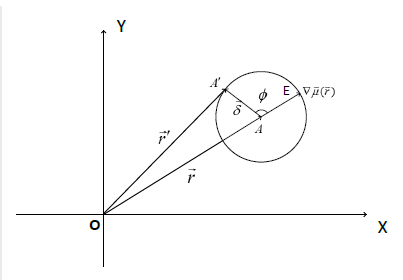
\includegraphics [width = 7cm]{Figure1.pdf}
%\vspace{-2 mm}
\caption{Description.}
\label{fig:1}
%\vspace{-5 mm}
\end{figure}

Figure 1 illustrates our model in two-dimension physical space. We designate the AP we sample as the original point $O$ of the coordinate system, and denote $A$ as as the user��s actual location which we focus on estimating. Assume that the distribution of RSS around $A$ are circular symmetric , therefore we can define region $E$ as a circle with radius $\delta$, and measurement in it means that the user is estimated at $A$ while outside it indicates at other possible locations rather than $A$. Note that if we consider any one of the straight lines through $A$, then the distribution and localization are identical to those in one-dimension situation. Then we define the vector from $O$ to $A$ in physical space as $\vec r$ and to any location $A'$ on the boundary of $E$ as $\vec r'$. Therefore, $\vec \delta  = \vec r' - \vec r$ in Figure 1 can be clearly deemed as the difference between user's real location and our estimation result, \ie, the accuracy of our localization. In addition, since $O$ is the AP we consider, the gradient of RSS at $A$ (\ie, $\nabla \vec \mu (\vec r)$ in Figure 1) must be the same direction as $\overrightarrow{OA}$. We also define $\varphi$ as the inserted angle between $\vec \delta $ and $\nabla \vec \mu (\vec r)$, $\varphi  \in \left( { - \pi ,\pi } \right]$, where $\varphi < 0$ denotes the absolute value of $\varphi$ is less than $\pi$ clockwise (\ie, starting from $\nabla \vec \mu (\vec r)$ to $\vec \delta $ while $\varphi  > 0$ indicates the opposite.

Similar as one-dimension condition, MLE can be the judgment of whether a user is located at $A$ in two-dimension physical space based on our localization system. For single-measurement situation the MLE can be expressed as:
\begin{align}
{f_{\vec r}}(P) \ge {f_{\vec r + \vec \delta }}(P),
\end{align}
where ${f_{\vec r}}(P)$ denotes the probability distribution function of RSS pertaining to the access point $P$ at location $\vec r$. However, unlike in one-dimension condition $\vec \delta$ is reduced to a scalar $\delta$ without directions ($\varphi$) taken into consideration, two-dimension problem requires MLE satisfy every single direction mapped by every possible value of $\varphi  \in \left( { - \pi ,\pi } \right]$. Hence, $\varphi$ should be embedded in our analysis.

In order to render our explanation simpler and clearer, we rotate the coordinate system to a point where the new x-axis covers $\overrightarrow{OA}$ (Figure 2). Meanwhile $\nabla \vec \mu (\vec r)$ is also co-linear with the x-axis. Then aiming to derive the specific expression of MLE, we firstly make some assumptions:
\begin{itemize}
\item[(1)] The radius value $\delta$ should be small enough since we intend to meet high localizing accuracy (distinguishing different locations with very short distances from each other). Therefore, $E$ can be viewed as a very small region in physical space.
\item[(2)] $\left| {\nabla \vec \mu (\vec r)} \right|$ equals to the difference between $\mu (\vec r + \vec \delta )$ and $\mu (\vec r)$ in which $\vec \delta $ is co-linear with the new x-axis. Hereinafter in this section we denote $\nabla$ as $\left| {\nabla \vec \mu (\vec r)} \right|$ to simplify the mathematical expression.
\item[(3)] Every line perpendicular to $\nabla \vec \mu (\vec r)$ represents that all locations on this line inside $E$ have uniform RSS value. Factually according to the direct correlation between distance and RSS, the equi-value delineation of RSS should be a circle rather than a straight line. Nevertheless, due to the fact that $E$ is small enough, the equi-value curve inside $E$ can be approximated as a line segment.
\item[(4)] The distribution of RSS strength in two-dimension physical space should be a two-dimension normal distribution. However given that every line vertical to the new x-axis represents an identical RSS value for all locations on it, the normal distribution is degraded to one dimension if we consider the distribution on the new x-axis.
\end{itemize}

It is clear that the RSS value of $\vec r$ (\ie, $\mu (\vec r)$) corresponds the largest measuring probability when $\vec r$ is which we aim to locate. \textbf{Original Graph in Section 4.1}. Hence we can derive
\begin{align}
{f_{\vec r}}(P) = \frac{1}{{\sqrt {2\pi } \sigma }}{e^{ - \frac{{{{(x - \mu (\vec r))}^2}}}{{2{\sigma ^2}}}}},
\end{align}
where $\sigma$ represents the intrinsic noise. Combining with Assumption 3 and 4, we can further derive ${f_{\vec r + \vec \delta }}(P)$ predicated on the representative condition in Figure 2.
\begin{align}
{f_{\vec r + \vec \delta }}(P) = \frac{1}{{\sqrt {2\pi } \sigma }}{e^{ - \frac{{{{(x - (\mu (\vec r) + \nabla \cos \varphi ))}^2}}}{{2{\sigma ^2}}}}}
\end{align}
Then to meet the conditions of MLE, we have:
\begin{align}
\frac{1}{{\sqrt {2\pi } \sigma }}{e^{ - \frac{{{{(x - \mu (\vec r))}^2}}}{{2{\sigma ^2}}}}} \ge \frac{1}{{\sqrt {2\pi } \sigma }}{e^{ - \frac{{{{(x - (\mu (\vec r) + \nabla \cos \varphi ))}^2}}}{{2{\sigma ^2}}}}}
\end{align}
for all $\varphi  \in \left( { - \pi ,\pi } \right]$. Simplify it we will have:
\begin{align}
{(x - \mu (\vec r))^2} \ge {(x - (\mu (\vec r) + \nabla \cos \varphi ))^2}
\end{align}
In order to gain clearer insight into this inequality, Figure 3 is displayed as follows in which the sample space is concerned.

In Figure 3, the endpoints of this line segment represent the extreme conditions that $\varphi$ equals to 0 and $\pi$. Analogical to one-dimension analysis, we can derive
\begin{align}
{P_{high}} = \frac{{\mu (\vec r) + (\mu (\vec r) + \nabla \cos \varphi )}}{2} = \mu (\vec r) + \frac{{\nabla \cos \varphi }}{2}\\
{P_{low}} = \frac{{\mu (\vec r) + (\mu (\vec r) - \nabla \cos \varphi )}}{2} = \mu (\vec r) - \frac{{\nabla \cos \varphi }}{2}
\end{align}
which evinces that our localizing estimation will be judged to $A$ if and only if $P$ satisfies ${P_{low}} \le P \le {P_{high}}$. Here we limit $\varphi  \in [ - \frac{\pi }{2},\frac{\pi }{2}]$ to ensure ${P_{high}} \ge {P_{low}}$, if $\varphi  \notin [ - \frac{\pi }{2},\frac{\pi }{2}]$ then we can exchange the expression of ${P_{high}}$ and ${P_{low}}$ to maintain ${P_{high}} \ge {P_{low}}$. \textbf{---Rule 1)} Since the \textbf{equality(n)} holds for any $\varphi  \in \left( { - \pi ,\pi } \right]$, thus if fall into all possible intervals $[{P_{low}},{P_{high}}]$ then it will be classified into location $A$. The extreme condition is that while $\varphi  = \frac{\pi }{2}$, ${P_{high}} = {P_{low}}$, indicating that $P$ will be judged to $A$ if and only if $P = {P_{high}} = {P_{low}}$. That is to say our measurement must estimate the user��s location exactly at $r$, the real location. However, as error exists all the time in measurement and estimation, it is practically impossible to reach this extreme condition. Since that our previous analysis cannot be directly applied to realistic problems.

\begin{figure}[!htbp]
\centering
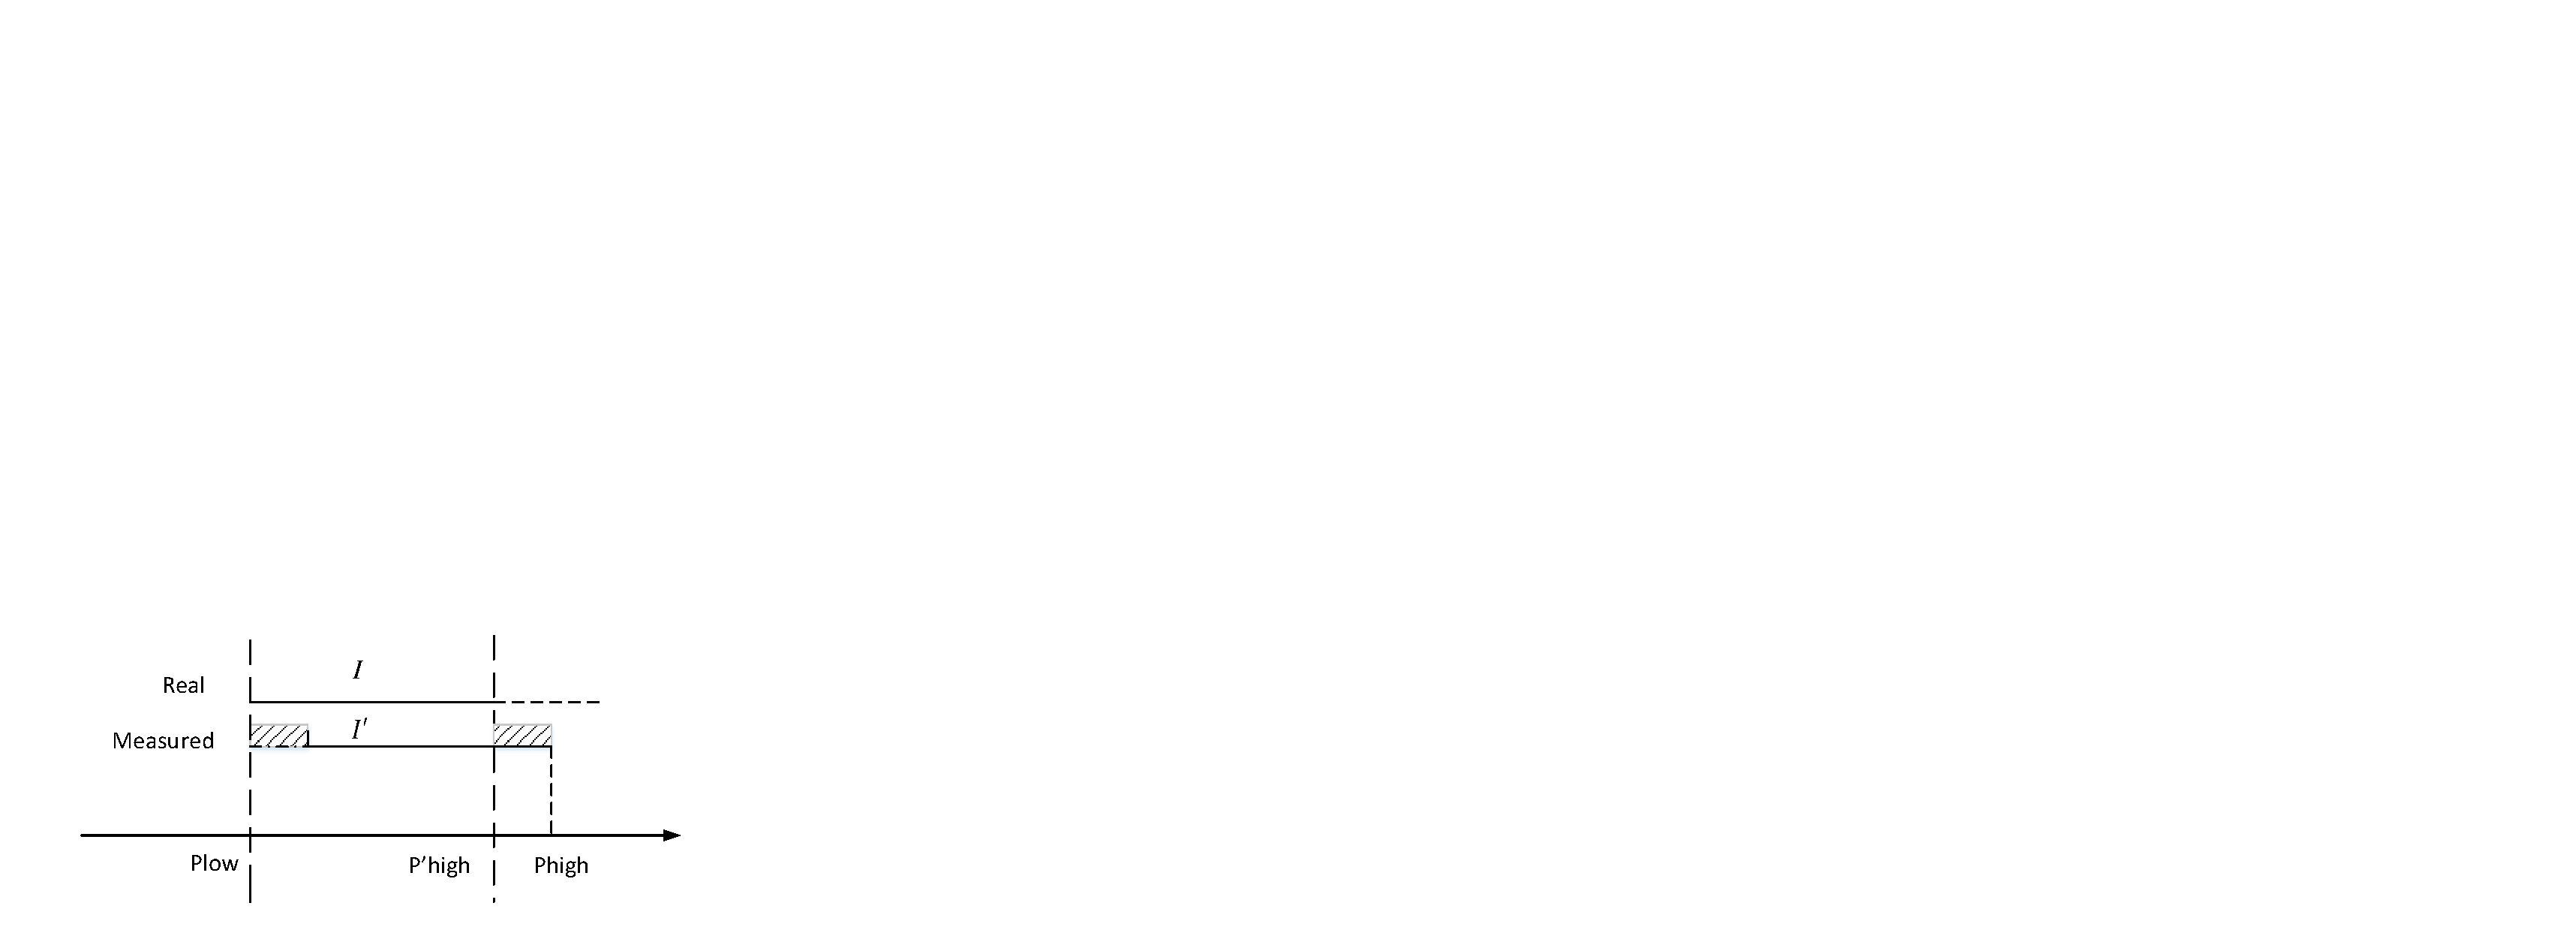
\includegraphics [width = 7cm]{Figure4.pdf}
%\vspace{-2 mm}
\caption{Description.}
\label{fig:4}
%\vspace{-5 mm}
\end{figure}

However, notice that practical indoor localization divides a room into many small square blocks and denotes the center of each block as a possible estimated location (\ie, if an estimation falls into one of these blocks, then the location we determine this user is the center of this block.) Therefore, it is not necessarily for us to consider all locations on the boundary of $E$ as analysis above. Instead we may solely concentrate on four blocks adjacent to our target block ($A$ is the center), and denote each center of these four block as $B, C, D, E,$ displayed in Figure 4. Under this circumstances, we will only have to meet four MLE constraints which relax our feasible solution from a single point $P$ to an interval. We will discuss it in detail with Figure 5.

Figure 5 is similar to Figure 3 and we define parameters in accordance with Figure 4. Then based on previous analysis we can easily write the simplified MLE constraints of $B, C, D, E$:
\begin{align}
\left\{\begin{array}{l}
{(x - \mu (\vec r))^2} \ge {(x - (\mu (\vec r) + \nabla \cos \phi ))^2}\\
{(x - \mu (\vec r))^2} \ge {(x - (\mu (\vec r) + \nabla \sin \phi ))^2}\\
{(x - \mu (\vec r))^2} \ge {(x - (\mu (\vec r) - \nabla \cos \phi ))^2}\\
{(x - \mu (\vec r))^2} \ge {(x - (\mu (\vec r) - \nabla \sin \phi ))^2}
\end{array}\right.
\end{align}
Therefore we can draw out Figure 6 in light of Figure 3. Then according to above analysis, it is clear that we can derive the feasible interval as
\begin{align}
I = \left[ {\mu (\vec r) - \frac{{\nabla \min \left\{ {\cos \phi ,\sin \phi } \right\}}}{2},\mu (\vec r) + \frac{{\nabla \min \left\{ {\cos \phi ,\sin \phi } \right\}}}{2}} \right]
\end{align}
where $\phi  \in \left[ { - \frac{\pi }{2},\frac{\pi }{2}} \right]$ and follows Rule 1. It demonstrates that a user is measured in block $A$ if and only if the estimation of him falls into $I$. Thus the reliability of our one-time measurement analysis of two-dimension physical space can be interpreted as:
\begin{align}
R = \int_{{P_{low}}}^{{P_{high}}} {{f_r}(P)dP = } \int_{\mu (\vec r) - \frac{{\nabla \min \left\{ {\cos \phi ,\sin \phi } \right\}}}{2}}^{\mu (\vec r) + \frac{{\nabla \min \left\{ {\cos \phi ,\sin \phi } \right\}}}{2}} {\frac{1}{{\sqrt {2\pi } \sigma }}{e^{ - \frac{{{{(x - \mu (\vec r))}^2}}}{{2{\sigma ^2}}}}}dx}
\end{align}

\subsubsection{Imperfect Data}
Then we extend our study to the influence of imperfect data in a two-dimension physical space. Recall in one-dimension analysis the imperfectness of received data is described as a deviation of line segment in the sample space. Therefore although our physical space has upgraded to two dimension, our sample space is still in one dimension as given above and what we receive are data of RSS, reflected directly in sample space. Thus we can imitate the method to derive error analysis similar as that of one-dimension situation.

We still set our target region as  and consider $A$ abut to $B, C, D, E$ abut to $A$. Firstly it is reasonable to assume that the probability that a user is located at any location in $A$ to be identical, so the distribution of user's true location in  is a uniform one, whose probability distribution function is:
\begin{align}
p{f_A}(Q) = \left\{ \begin{array}{l}
\frac{1}{S},\quad Q \in A\\
0,\quad Q \notin A
\end{array} \right.
\end{align}
where $A$ denotes the target region, $S$ represents its area and $Q$ means a user's true location. Note that every $Q$ in two-dimension physical space can be mapped to the one-dimension sample space according to Assumption 3. Now we set the user's true location in physical space is ${Q_0}$ and its corresponding point in sample space is $X_0$. Figure 7 illustrates the influence of imperfectness of data procured, which results in the deviation of feasible interval $I$ in sample space from its true range. As in Figure 7 we denote the right endpoint of true range as $X_1$ and deviated range as $X_2$, hence we can discover if a point $X_0$  falls into interval $(X_1,X_2)$, then it will be falsely estimated: $X_0$ should have been classified into region $B$ while because of the deviation it is determined to be in region $A$. The same goes for the left side of region $A$, the boundary point of $A$ and $C$. Given our situation, then we can derive the probability of localizing error as:
\begin{align}
P(err) &= \iint_A {{f_A}}(Q)P(err|X = {X_0})dxdy\\
&= 2\iint_A {{f_A}}(Q)\int_{{X_1}}^{{X_2}} {\frac{1}{{\sqrt {2\pi } \sigma }}{e^{ - \frac{{{{(X - {X_0})}^2}}}{{2{\sigma ^2}}}}}} dXdxdy
\end{align}










\section{Characterization of Data Quality and Localization Error}

\subsection{Data Quality}

\subsubsection{The philosophy of using Fisher Information as metric}

\subsection{Data Aggregation}%Building fingerprint database  with purchased data

\subsection{Localization Error}

\section{regret minimization}

\section{truthful}

\subsection{Solution}
?
\subsection{Price of Truthful}


\section{Fingerprint Database Update}

\subsection{Problem Formulation}

\subsection{Algorithm and Analysis}

\section{Experiment Results}

\section{Related works}

\section{Conclusion}
The conclusion goes here.
\begin{comment}
\begin{figure}[!htbp]
\centering
\includegraphics [width = 7cm]{.//pic//HistEncryptionDE.eps}
%\vspace{-2 mm}
\caption{Computation overheads of encryption, decryption, and escrow-decryption per data owner.}
\label{fig:EncryptionDE}
%\vspace{-5 mm}
\end{figure}
\end{comment}






%


%\appendices
%\section{Proof of the First Zonklar Equation}
%Appendix one text goes here.
%
%
%\section{}
%Appendix two text goes here.
%
%
%\section*{Acknowledgment}
%
%
%The authors would like to thank...
%
%
%\ifCLASSOPTIONcaptionsoff
%  \newpage
%\fi
%
%
%
%
%\begin{thebibliography}{1}
%
%\bibitem{IEEEhowto:kopka}
%H.~Kopka and P.~W. Daly, \emph{A Guide to \LaTeX}, 3rd~ed.\hskip 1em plus
%  0.5em minus 0.4em\relax Harlow, England: Addison-Wesley, 1999.
%
%\end{thebibliography}
%
%%
%
%\begin{IEEEbiography}{Michael Shell}
%Biography text here.
%\end{IEEEbiography}
%
%\begin{IEEEbiographynophoto}{John Doe}
%Biography text here.
%\end{IEEEbiographynophoto}
%
%
%
%\begin{IEEEbiographynophoto}{Jane Doe}
%Biography text here.
%\end{IEEEbiographynophoto}
%
%

\end{document}


